\chapter{Contributions}
\label{sec:contributions}
\fixme{All subsections need to be expanded and further clarified.}

In this section we will tie together the different publications made during the course of the PhD studies. We will focus on the general message of the publications in relation to the goal of the PhD. We remand to the full text of the individual publications in Appendices~ \ref{sec:glass}-\ref{sec:vrbrdf} for the full technical details.

\section{Outline and motivation}

(Figure: Fields in which we need instant feedback on appearance: 3d printing, artist feedback, quality control, meat)

As we discussed in Chapters~\ref{sec:background} and~\ref{sec:related}, many efforts have been put forward by the community to allow interactive physically based rendering. We barely scratched the surface on reporting these techniques in Section~\ref{sec:related}, that are becoming widely popular in recent years due to increasing GPU power. 

We argue that there is a need in the industry for photorealistic accurate interactive rendering. In many fields, people need immediate feedback on how the rendering will actually look. Some examples include visual inspection of produced parts, previews of 3D printed objects, artistic iterations for movie scenes, and prediction of appearance after a production process. These various applications define a photorealistic-interactive spectrum, depending how close to a physically based vs. how fast the rendering is. Our contributions over the course of the PhD studies place themselves at different points across this spectrum.

Our contribution~\ref{sec:juice} provides a first example on why we need both fast and accurate rendering, in the form of estimating scattering parameters of cloudy apple juice. In this paper and in contribution~\ref{sec:glass} we discuss on what is photorealistic rendering, and how good it should be to allow parameter estimation. We will move then towards the interactive end of the spectrum, discussing our technique for interactive directional subsurface scattering. We will finally discuss two applications at the other end of the spectrum, one leveraging recent innovations in interactive ray tracing to solve a common problem in real time graphics, and one leveraging physically based materials in a hard real time physically based application. 

\section{Defining photorealistic rendering}
\begin{figure}
\begin{tabular}{@{}c@{}c@{}}
	 \includegraphics[height=4.3cm]{figures/comparison} & \hspace{2em}
	 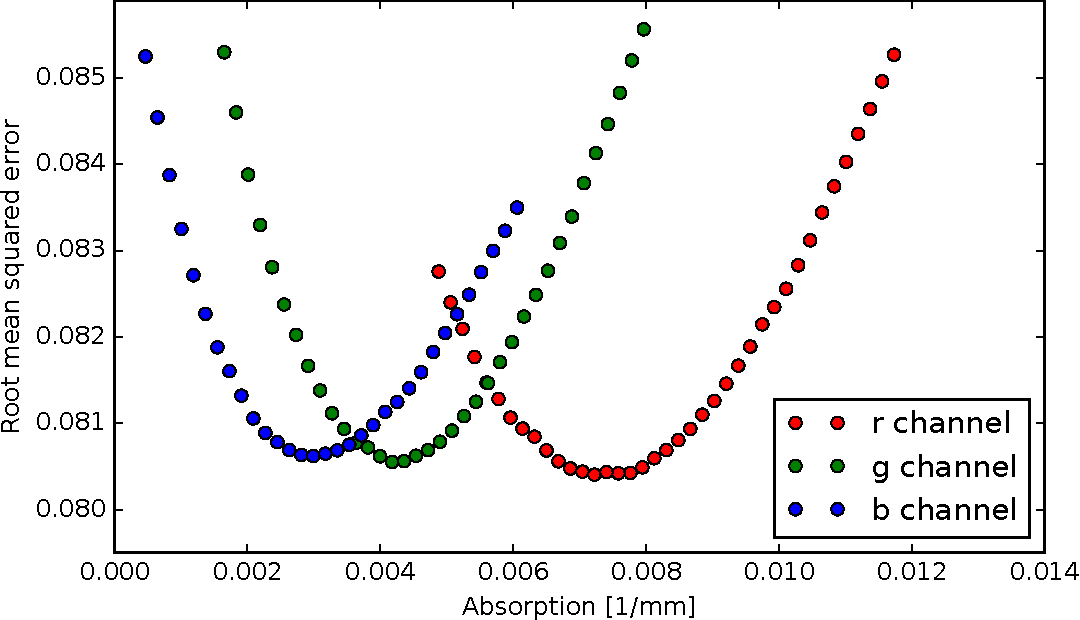
\includegraphics[height=4.3cm]{figures/glass_bowl_analysis_by_synthesis}  \\
\end{tabular}
\caption{\fixme{Write me.}} %The red rectangle shows where we estimated RMSE in Table \ref{table:quant}.}
\label{fig:glasscomparison}
\end{figure}

There is a difference tough between \emph{physically based} and \emph{photorealistic} rendering. In the former, the emphasis is onto creating rendering models and techniques that are based on physical radiometric processes. In the latter, we put emphasis on \emph{validating} the models with real images (see Figure~\ref{fig:juicecomparison}). Our first contributions~\ref{sec:glass} and~\ref{sec:juice} set out to test physically based rendering. The question is: how good is photorealistic rendering when compared to actual images?

Two investigations led to a number of interesting insight on physically based rendering. A first insight is that renderings and pictures can be compared, and actual physical quantities can be measured from them (See Figure~\ref{fig:glasscomparison}). In our first contribution, we identified a number of different challenges in comparing pictures and renderings, mostly related to the scene. The task is also made more difficult if the material is of a kind that influences its surroundings, like scattering (e.g. juice) or absorbing (e.g. impure glass) media. 

\begin{figure}
\begin{tabular}{@{}c@{}c@{}}
	 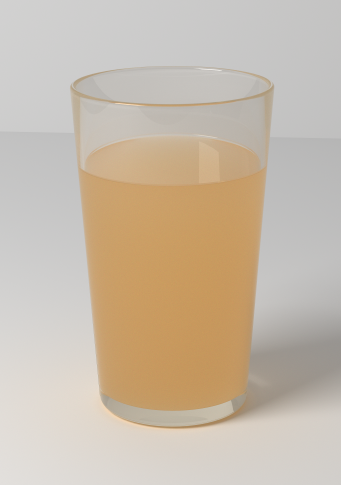
\includegraphics[width=0.5\columnwidth]{figures/teaser_render.png} &
	 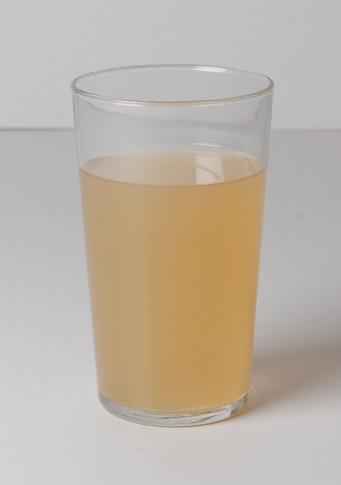
\includegraphics[width=0.5\columnwidth]{figures/ref_img.jpg}  \\
	rendering & photograph \\
\end{tabular}
\caption{Cloudy apple juice photographed and rendered using our appearance model. In the model, apple particle concentration (0.8 g/l) and apple storage period (4 days) were selected to match the photograph.} %The red rectangle shows where we estimated RMSE in Table \ref{table:quant}.}
\label{fig:juicecomparison}
\end{figure}

We set out to solve this challenge in our main contribution~\ref{sec:glass}. While we successfully compared renderings and images to a degree that was not possible before, it requires a great number of steps and attention to details to make sure the geometry of both scene and objects match. As we can see from Figure~\ref{fig:glasscomparison}, we are able to measure material properties like the spectral absorption coefficient $\sigma_a$. This ability of compare would allow in the future to further improve existing techniques in acquisition, rendering and reconstruction. If the quality of the reconstruction becomes good enough, even path tracing could be compared with the original image.

%Take home points:
%\begin{itemize}
%\item Preliminary study: appearance prediction is important, interactivity is important.
%\item Realistic reconstruction is hard. 
%\item At the moments, it is not possible to evaluate how good path tracing is.
%\item Tough, we can evaluate and measure parameters from the scene. Being able to compare is what it is all about.
%\item Fine details make the difference, especially in geometry
%\item Identify problems in acquisition, rendering and reconstruction, using the dataset to improve current rendering techniques.
%\item Publicly available dataset?
%\end{itemize}

\section{Interactive rendering of scattering media}
\begin{figure}
\begin{tabular}{@{}c@{$\,$}c@{}c@{}c@{}}
& directional dipole, 6 fps & standard dipole and VPLs \\
\begin{sideways}\hspace*{1.5em}our method\end{sideways} &
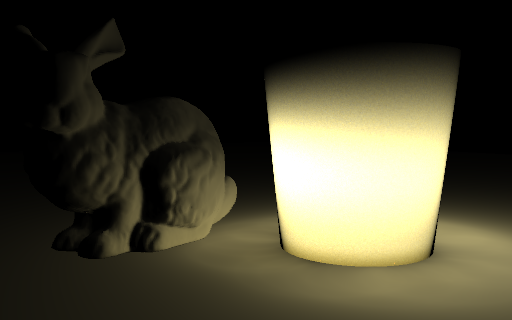
\includegraphics[width=0.48\columnwidth]{figures/candle_holder_directional_6fps.png} &
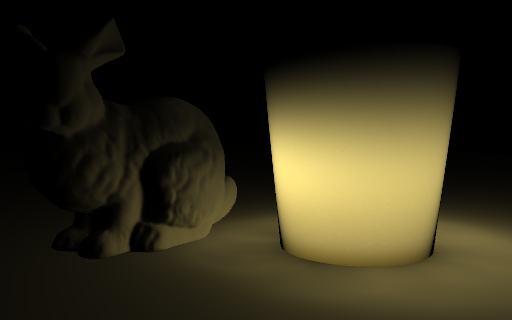
\includegraphics[width=0.48\columnwidth]{figures/candle_holder_jensen_converged.png} \\[-4pt]
\begin{sideways}\hspace*{1.7em}ray tracer\end{sideways} &
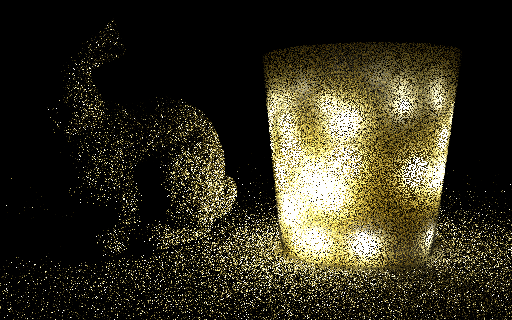
\includegraphics[width=0.48\columnwidth]{figures/scene_comparison_optix_6fps.png} &
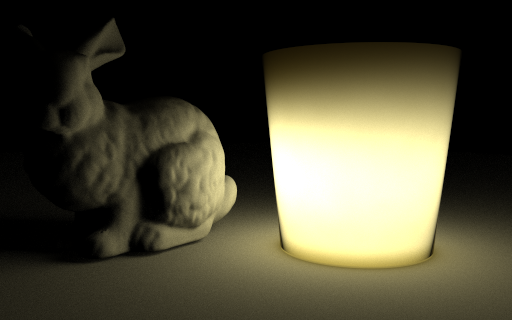
\includegraphics[width=0.48\columnwidth]{figures/scene_comparison_converged.png} \\[-0.5ex]
& directional dipole, 6 fps & directional dipole, reference \\[-1ex]
\end{tabular}
\caption{Equal time comparison (left column) of our method with the reference method and qualitative comparison with diffuse subsurface scattering (upper right) and the converged reference solution (lower right). The scene is lit by a point light in a white grapefruit candle holder.} % Emerging light illuminates a diffuse Stanford Bunny on a tabletop.}
\label{fig:optixcomparison}
\end{figure}

After discussing photorealism in the previous section, in this section we start discussing how to bring photorealistic rendering into the interactive domain, namely in the specific case of rendering translucent materials. 

Contribution~\ref{sec:interactivedirsss} describes an interactive techniques on GPUs for rendering translucent materials. The most important contribution in this technique is that allows rendering using \emph{directional} BSSRDFs like the one proposed by TODO. The directional dipole is a recent analytical model where the BSSRDF depends on $\vec{\omega}_i$, the direction of the incoming light. This allows more subtle scattering effects to be computed, accounting partially for the single scattering component in the scattering process. See Figure~\ref{fig:optixcomparison}, top row, for a comparison between the standard and the directional dipole. Many of the previous interactive techniques for rendering BSSRDFs assume that the BSSRDF can be represented as a function of only one variable (i.e. the distance between the point of incidence and emergence). This can be exploited for different optimizations, like filtering, precomputation or tabulation. 

Our technique leverages the strengths of rasterization as a rendering techniques, storing progressive maps of scattered radiosity rendered from different directions around the object. This particular configuration allows us to contribute with a fully interactive technique, that does not require neither precomputation nor texture parameterization. Given this features, we can apply this technique to procedural deformable objects, something that is generally quite difficult to achieve with precomputation techniques.

As another contribution of our technique, we leverage our scattered radiosity maps to place virtual point lights on the surface of the objects. This allows to transfer emergent light onto other surfaces. An example can be seen in Figure~\ref{fig:optixcomparison}, where we transport the light from a point light inside an object on the outside, illuminating the bunny on the tabletop. In the same figure, we can see on how we successfully compare to a fully path traced simulation (bottom right) that in the same time we render our solution cannot achieve the same results, looking unconverged and noisy (bottom left).

%\begin{itemize}
%\item cloudy apple juice study.
%\item Rouch estimate during production
%\item It is possible to apply complicated rendering models (like directional SSS) in an interactive domain
%\item Working under constraints
%\item Texture-free, deformable model
%\item Leveraging the strength of rasterization
%\item Multiple lights
%\item Global illumination extensions: how you do reuse information that you have already available
%\item Maps of scattered radiosity
%\item Progressive rendering
%\item Interactive transport of emergent light from deformable objects
%\item Transport of light behind translucent objects.
%\end{itemize}

\section{Interactive stable ray tracing}
\begin{figure}
\begin{tabular}{@{}c@{}c@{}@{}c@{}}
	 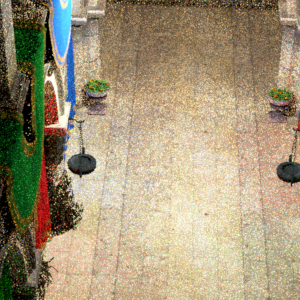
\includegraphics[width=0.33\textwidth]{figures/ss_2x_rect_370_300_300_300_frame_211.png} &
		 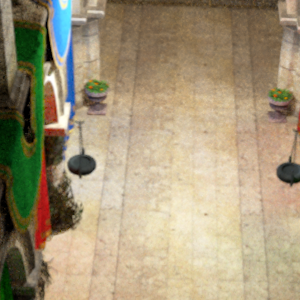
\includegraphics[width=0.33\textwidth]{figures/ss_2x_taa_rect_370_300_300_300_frame_211.png} &
		  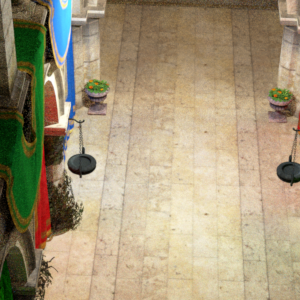
\includegraphics[width=0.33\textwidth]{figures/ss_32x_rect_370_300_300_300_frame_211.png} \\	 
Supersampling, 2 spp & Supersampling, 2 spp 	& Supersampling, 32 spp \\
  					 & + temporal antialiasing 	&  \\
sharpness: 0.7924 & sharpness: 0.5348 & sharpness: 0.6771  \\
	 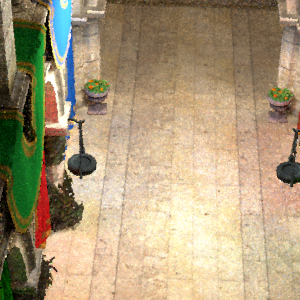
\includegraphics[width=0.33\textwidth]{figures/srt_1_rect_370_300_300_300_frame_211.png} &
	 	 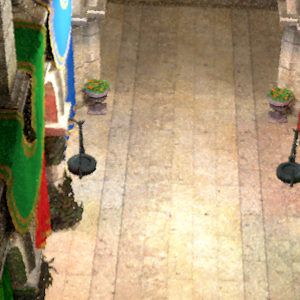
\includegraphics[width=0.33\textwidth]{figures/srt_1_ti_rect_370_300_300_300_frame_211.png} &
	  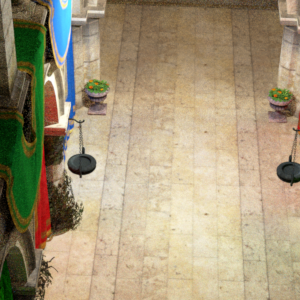
\includegraphics[width=0.33\textwidth]{figures/ss_32x_rect_370_300_300_300_frame_211.png}
 \\
Stable ray tracing, 1 spp & Stable ray tracing, 1 spp & Supersampling, 32 spp \\
 & + temporal integration &  \\
sharpness: 0.7085 & sharpness: 0.6060 & sharpness: 0.6771 \\[-1.5ex]
\end{tabular}
\caption{Including indirect illumination, the different techniques are here applied to a frame in the Sponza video.}
\label{fig:sponza_video_frame}
\end{figure}

After dealing with subsurface scattering, we explored the spectrum of interactive-photorealistic techniques one step further in paper~\ref{sec:srt}. As in the previous section, we use caching as a technique to improve existing physically based techniques. In this contribution, in particular, we discuss temporal stability over the context of interactive ray tracing. When going to a real time domain, the number of paths we can shoot per pixel becomes extremely limited. Also, the shading locations change every frame, causing a noisy image, both spatially and temporally. Existing techniques, namely temporal anti aliasing, can mitigate the problem, tough introducing blur. By recycling shading locations between frames, we can improve temporal stability, while retaining sharpness. We can see the results in Figure~\ref{fig:sponza_video_frame}. The main contribution on this technique is to provide a system to improve temporal stability: any other technique can be further applies on top to further improve shading quality. 

Another contribution of this technique is that it shows how we can leverage the strength of one interactive technique, namely ray tracing, against the most commonly used rasterization. Current hardware does not allow shading locations to be arbitrarily chosen within a pixel. In our technique, we allow shading location to vary in screen space per pixel, while staying the same in world space.

Another advantage of this technique, in particular in a photorealistic rendering context, is that it allows to store shading information across frames, e.g. to store indirect illumination. This will allow in the future to extend the technique with other sort of data, to further improve the technique. 
%
%\begin{itemize}
%\item Take home message: recycling information can be useful to improbe temporal stability 
%\item Leveraging ray tracing strengths against rasterization
%\item Reprojection 
%\item Sharp and antialiased
%\item Application to photorealistic rendering in the form of indirect global illumination
%\item Foundation technique to combine with existing ones
%\item Spatial aliasing
%\item Good results with progressive path tracing.
%\end{itemize}

\section{Applying interactive photorealistic techniques}
\begin{figure}
\centering
\begin{tabular}{@{}c@{}c@{}}
	 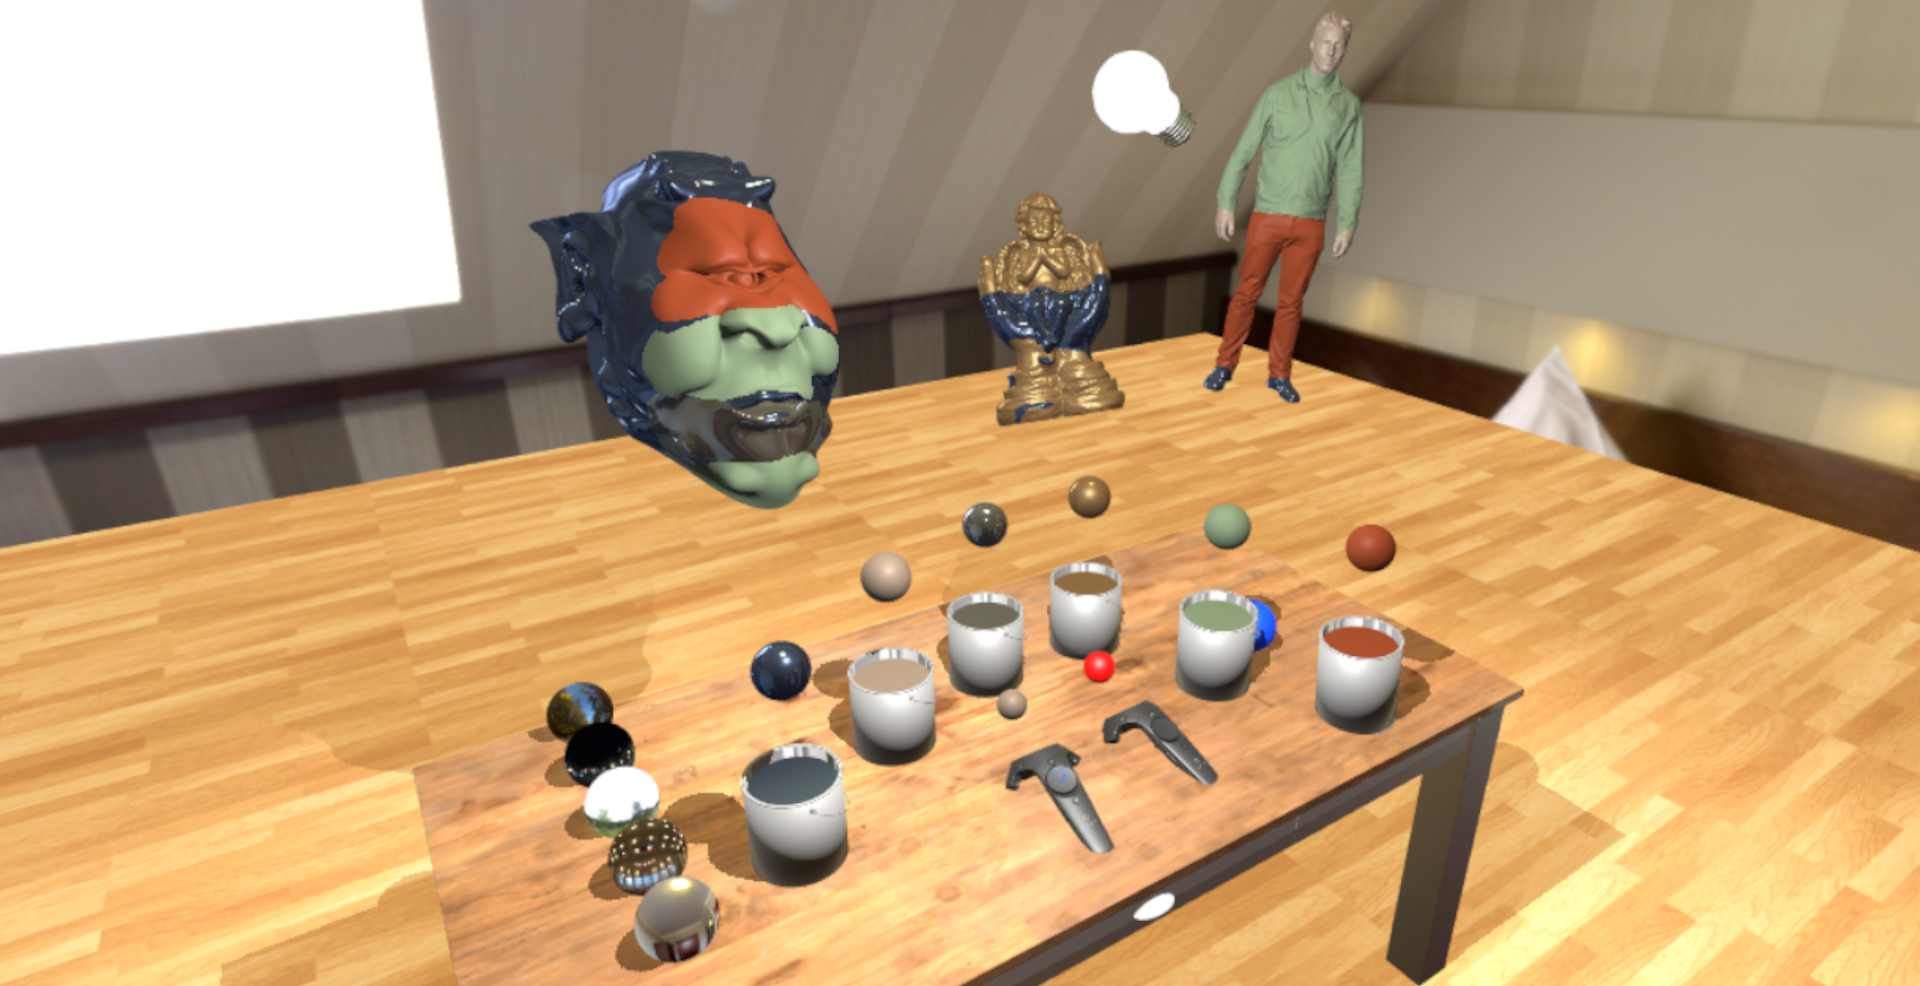
\includegraphics[height = 4.3cm]{figures/screen1_crop} &
		 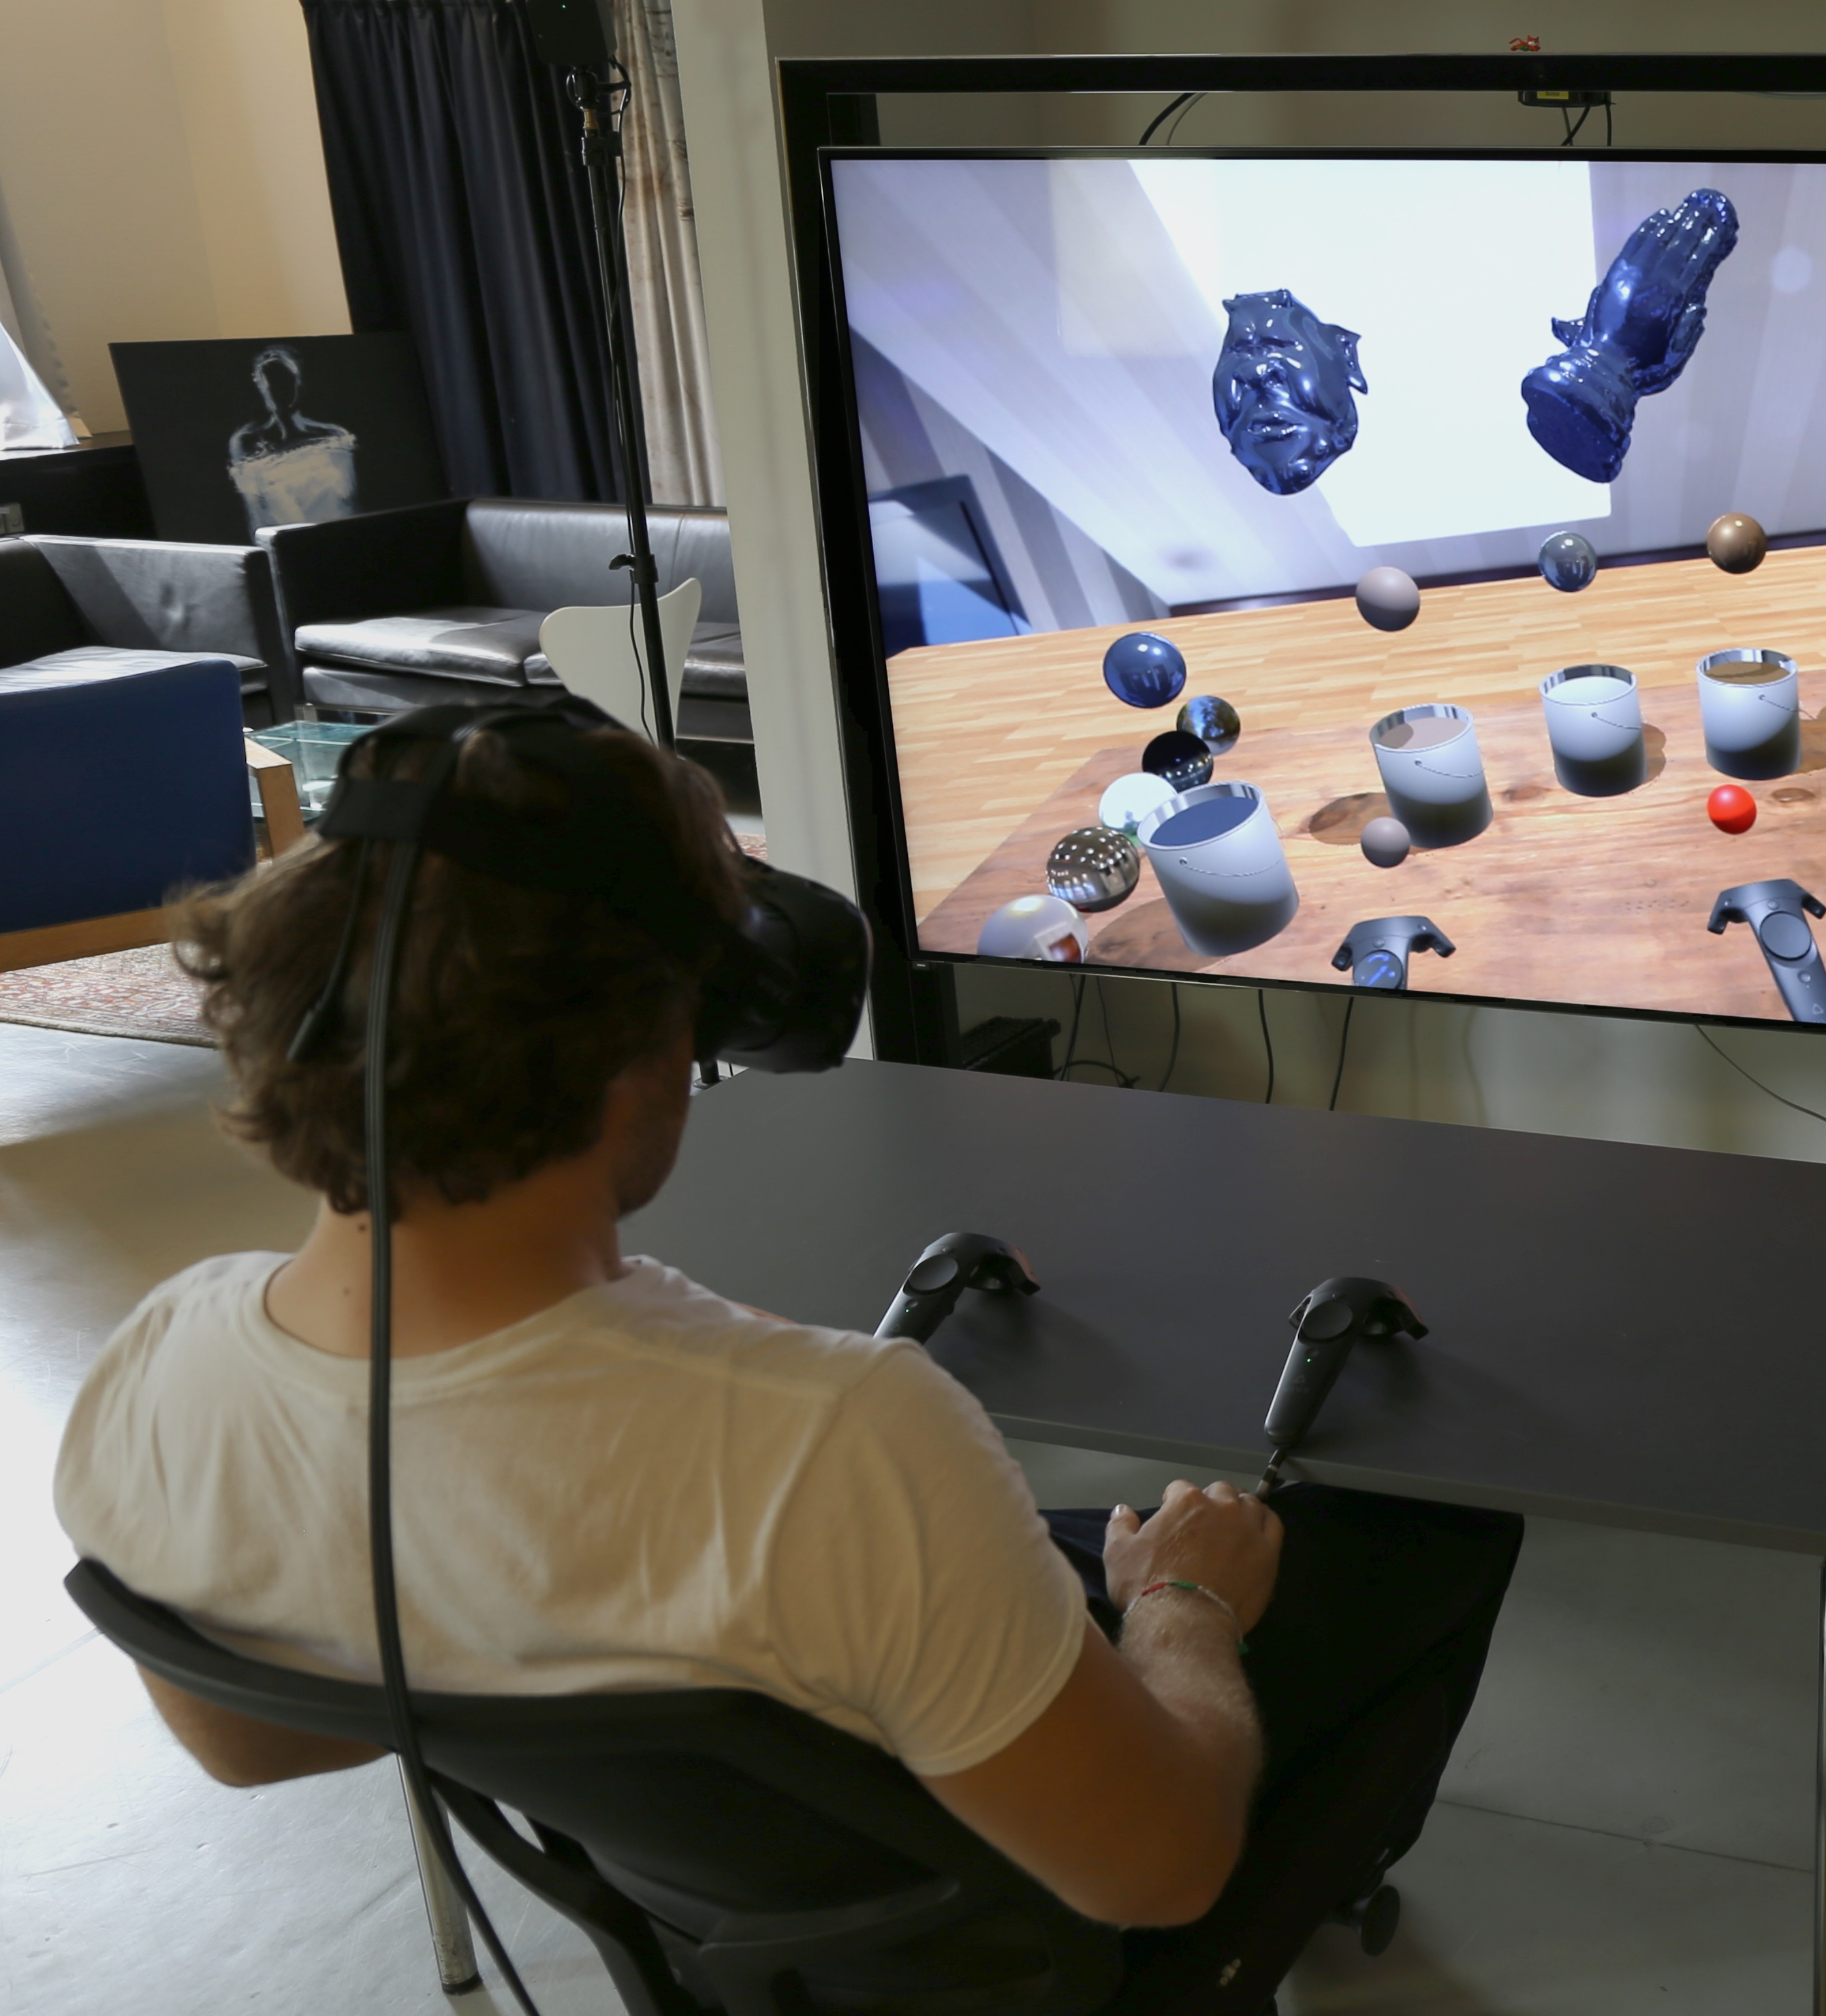
\includegraphics[height = 4.3cm]{figures/person} \\[-2.5ex]
\end{tabular}
  \caption{Pictures illustrating our VR demo application, with an in-game screenshot (left) and a picture of the setup (right). }
  \label{fig:vrbrdfimage}
\end{figure}
In contribution~\ref{sec:vrbrdf}, we push phisically based rendering even further, applying it to a so-called hard real time environment, virtual reality. I nthis context, applications need to consistently perform over 90 frames per seconds, in order to avoid issues for the users, e.g. motion sickness. In our application, we modify an existing engine pipeline to include phisically based BRDFs, in the discretized form of the MERL database. This proof of concept was born as an inspecting tool to debug physically based materials, aided by the provided in game controllers (see Figure~\ref{fig:vrbrdfimage}). The application gives a glimpse into the future, showing how photorealistic materials augment the immersion of the application by allowing a virtual world that is more similar to the real one. 

%\begin{itemize}
%\item Application to photorealisitic rendering to hard real time constratins
%\item Hint at future work that can be done
%\item Practical purpose: debug acquired BSRDF models.
%\item Apply real time techniques
%\item More constraints.
%\end{itemize}

\section{Discussion}